\chapter{INTRODUCTION}

This chapter explains the aim and scope of the research, including the background, problem statement, objectives, significance, conceptual framework, scope and limitations, and definition of terms.

\section{Background of the Study}

Road infrastructure quality fundamentally determines a nation's economic efficiency and public safety. Among pavement distresses, potholes represent one of the most critical and rapidly developing defects, directly impacting vehicle safety, infrastructure longevity, and maintenance economics. Globally, potholes impose substantial economic burdens. In the United States, pothole-related vehicle damage cost drivers an estimated \$26.5 billion in 2021 alone, with an average repair cost of approximately \$600 per incident \textcite{AAA2021}. Poor road conditions also contribute to increased vehicle emissions, accelerated tire wear, and higher accident risks \textcite{Burningham2005}.

The management of road infrastructure, particularly pothole detection and repair, directly supports multiple United Nations Sustainable Development Goals (SDGs), including SDG 9 (Industry, Innovation, and Infrastructure), SDG 11 (Sustainable Cities and Communities), and SDG 3 (Good Health and Well-being) by promoting resilient infrastructure, reducing traffic fatalities, and enhancing urban sustainability.

In the Philippines, road transport accounts for over 98\% of passenger transportation and a significant portion of freight movement \textcite{ADB2012}. The national road network spans approximately 35,164 kilometers, supporting a rapidly growing vehicle fleet. This escalating demand intensifies pressure on road infrastructure, making efficient pothole detection and quantification essential for sustainable management.

The Department of Public Works and Highways (DPWH) mandates a strict 3-working-day response time for pothole repairs, recognizing them as imminent safety hazards. However, conventional Road Condition (RoCond) assessments remain predominantly manual, time-consuming, and costly at approximately Php 4,000 per kilometer \textcite{Ramos2022}. This creates significant latency between detection and intervention.

Beyond detection, accurate surface area estimation is critical for maintenance economics, enabling precise material quantity forecasts, severity-based prioritization, and budget optimization. Traditional methods rely on subjective visual estimates, leading to material waste or shortages \textcite{Ramos2022}.

Current automated solutions often rely on 2D object detection, which cannot provide physical dimensions without depth information. High-fidelity 3D sensing technologies such as LiDAR remain prohibitively expensive for widespread deployment in developing contexts.

Recent advances in monocular metric depth estimation (MMDE) offer a transformative, low-cost alternative by inferring accurate metric depth from single RGB images. Among these advances, Depth Anything V2 (DA2) represents a state-of-the-art foundation model capable of robust, high-fidelity depth inference across diverse environments. When integrated with real-time detection models like YOLOv10 and geospatial tagging, this enables end-to-end pothole surface area estimation in real-world coordinates.

Despite these technological advances, no existing study has integrated monocular metric depth estimation with real-time object detection specifically for pothole surface area quantification in tropical road environments. This research gap motivates the development of Eyeway 2.0, a vehicle-mounted AIoT system that combines YOLOv10 for pothole localization with Depth Anything V2 for monocular depth-based surface area quantification and GPS-enabled geospatial visualization, thereby addressing key gaps in Philippine road maintenance practices.

\section{Statement of the Problem}

The challenge of road maintenance in the Philippines is exacerbated by limitations in current methodologies. This research addresses the following problems: (1) manual inspections are too slow to support DPWH's rapid response mandates, while many automated 2D systems lack quantitative metrics \textcite{Ramos2022}; (2) without metric depth, systems cannot estimate pothole surface area in real-world units ($cm^2$ or $m^2$), hindering accurate material planning and severity prioritization; (3) precise 3D scanning technologies are unaffordable for routine municipal use; (4) tropical conditions (water-filled potholes, glare, shadows) degrade vision-based performance; and (5) lack of geospatial mapping prevents actionable intelligence for maintenance dispatch.

\section{Objectives of the Study}

The general objective of this study is to design, develop, and evaluate Eyeway 2.0, an integrated AIoT system for automated pothole surface area estimation and geospatial visualization deployed on a GPU-enabled edge device.

The specific objectives are as follows:

\begin{enumerate}
  \item To design and develop a pothole detection module using YOLOv10 optimized for edge deployment.
  \item To implement monocular depth estimation with Depth Anything V3 and convert depth maps to real-world surface area measurements using camera geometry.
  \item To create a geospatial visualization platform that displays GPS-tagged potholes with quantitative surface area metrics and severity indicators.
  \item To evaluate system performance in terms of detection accuracy (mAP), surface area estimation error (MAE and RMSE), and processing speed (FPS) under actual Philippine road conditions.
\end{enumerate}

\section{Significance of the Study}

Eyeway 2.0 enables a critical shift from reactive to data-driven, severity-based maintenance. By automating pothole surface area estimation, this study delivers significant contributions to the following sectors:

\begin{enumerate}
  \item \textbf{Department of Public Works and Highways (DPWH) and Local Government Units (LGUs):} The system supports regulatory compliance and optimizes fiscal planning through accurate material estimates. Furthermore, it enhances administrative accountability by digitizing the damage assessment process.

  \item \textbf{Road Users:} The deployment of this system contributes to a reduction in vehicle damage and accident rates by accelerating repair response times, thereby supporting the goals of SDG 3 (Good Health and Well-being) and SDG 11 (Sustainable Cities and Communities).

  \item \textbf{Researchers:} This study validates the novel application of monocular depth estimation models, specifically Depth Anything V3, for infrastructure metrology within tropical environments.

  \item \textbf{Society at Large:} The project democratizes advanced monitoring technology, ensuring that rural and secondary road networks receive equitable attention and maintenance resources compared to major thoroughfares.
\end{enumerate}

\section{Conceptual Framework}

The conceptual framework of this study, illustrated in Figure \ref{fig:conceptual-framework}, presents the hypothesized relationships between the key variables. The independent variable is the Hybrid AIoT Architecture of Eyeway 2.0, which integrates YOLOv10 for pothole detection, Depth Anything V2 for monocular depth estimation, and a geospatial module for location tagging and visualization. This architecture is posited to directly influence three dependent variables: (1) detection accuracy, measured by mean Average Precision (mAP); (2) measurement precision, evaluated through Mean Absolute Error (MAE) and Root Mean Square Error (RMSE) of estimated pothole surface area; and (3) system efficiency, assessed via processing speed in Frames Per Second (FPS) and overall resource consumption.

The strength and direction of these relationships are moderated by three external factors: ambient lighting conditions, accuracy of camera calibration parameters (intrinsic and extrinsic), and uniformity of road surface texture. Prior studies have established that lighting variability significantly affects object detection performance in outdoor environments \textcite{Arya2021}, while camera calibration accuracy directly impacts metric depth estimation fidelity \textcite{Koch2015}. Road surface texture uniformity influences both pothole boundary delineation and depth map quality \textcite{Majidifard2020}. These moderating variables affect how effectively the Hybrid AIoT Architecture performs under real-world Philippine road conditions.

\begin{figure}[ht]
    \centering
    \resizebox{\textwidth}{!}{%
    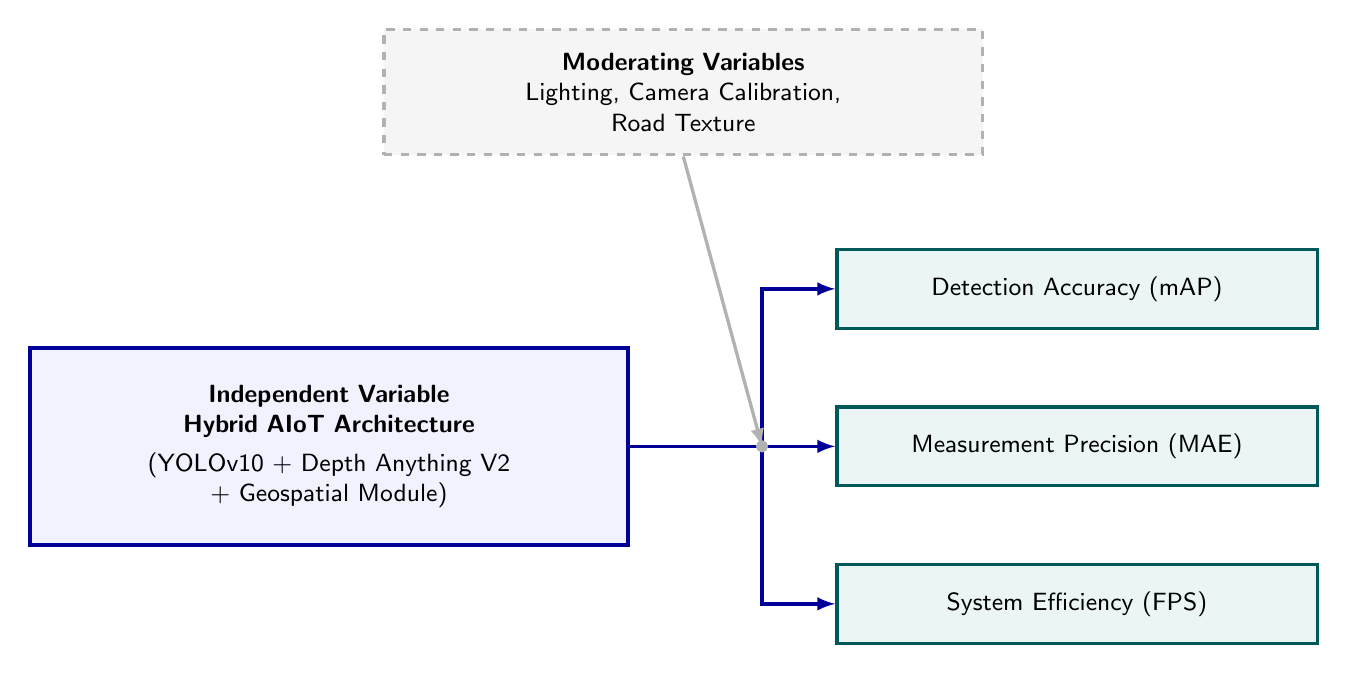
\begin{tikzpicture}[
        % Professional Style with Colors
        node distance=2cm,
        every node/.style={font=\sffamily\small},
        % Box Styles
        basebox/.style={
            rectangle,
            thick,
            fill=white,
            align=center,
            inner sep=3mm
        },
        ivbox/.style={
            basebox,
            draw=blue!60!black, % Independent Variable Blue
            fill=blue!5,
            line width=1.5pt,
            text width=7cm,
            minimum height=2.5cm
        },
        dvbox/.style={
            basebox,
            draw=teal!70!black, % Dependent Variable Teal
            fill=teal!8,
            line width=1.2pt,
            text width=5.5cm,
            minimum height=1cm
        },
        modbox/.style={
            basebox,
            draw=gray!60, % Moderating Variable Gray
            fill=gray!8,
            line width=1.2pt,
            text width=7cm,
            minimum height=1.5cm,
            dashed
        },
        % Connector Styles
        arrow/.style={-latex, line width=1.2pt, draw=blue!60!black},
        modarrow/.style={-latex, line width=1.2pt, draw=gray!60}
    ]
    
    % --- Moderating Variables (Top) ---
    \node[modbox] (mod) at (4.5, 4.5) {
        \textbf{Moderating Variables}\\
        Lighting, Camera Calibration,\\Road Texture
    };
    
    % --- Independent Variable (Left) ---
    \node[ivbox] (iv) at (0, 0) {
        \textbf{Independent Variable}\\
        \textbf{Hybrid AIoT Architecture}\\[3pt]
        (YOLOv10 + Depth Anything V2\\+ Geospatial Module)
    };
    
    % --- Dependent Variables (Right) ---
    \node[dvbox] (dv1) at (9.5, 2)  {Detection Accuracy (mAP)};
    \node[dvbox] (dv2) at (9.5, 0)  {Measurement Precision (MAE)};
    \node[dvbox] (dv3) at (9.5, -2) {System Efficiency (FPS)};
    
    % --- Paths & Connections ---
    
    % Define the "main effect" junction point
    \coordinate (junction) at (5.5, 0);
    
    % Draw lines from IV to junction area, then split to DVs
    \draw[arrow] (iv.east) -- (junction) |- (dv1.west);
    \draw[arrow] (iv.east) -- (dv2.west);
    \draw[arrow] (iv.east) -- (junction) |- (dv3.west);
    
    % Draw Moderating Arrow
    \draw[modarrow] (mod.south) -- (junction);
    % Interaction dot
    \filldraw[gray!60] (junction) circle (2pt);
    
    \end{tikzpicture}%
    }
    \caption{Conceptual framework illustrating the Hybrid AIoT Architecture influencing detection accuracy, measurement precision, and system efficiency, moderated by environmental and calibration factors.}
    \label{fig:conceptual-framework}
\end{figure}

\section{Scope and Limitations}

\subsection{Scope}
The study focuses on surface area estimation of potholes on paved asphalt and concrete roads using a single monocular RGB camera. Data collection will be conducted on national and provincial roads within the Metropolitan Manila and Central Luzon regions of the Philippines. The system employs YOLOv10 for pothole detection and Depth Anything V2 for scene depth estimation to derive surface area in real-world coordinates via perspective geometry and camera parameters. GPS integration enables geospatial mapping of detected defects. The system is designed for pothole surface area estimation only; it does not measure pothole depth (vertical dimension) or predict future road deterioration.

\subsection{Limitations}
Water-filled potholes may obscure surface geometry, leading to underestimation of area; such instances will be documented through annotation of affected samples. The system requires a GPU-enabled edge device for efficient processing. Accuracy is highly dependent on proper camera calibration and stable vehicle mounting. Performance may degrade under extreme low-light conditions or heavy occlusion.

\section{Definition of Terms}
\begin{description}
  \item[AIoT (Artificial Intelligence of Things)] The integration of artificial intelligence technologies with Internet of Things infrastructure to enable intelligent, autonomous decision-making in connected devices.

  \item[Depth Anything V2 (DA2)] A state-of-the-art foundation model for robust, high-fidelity monocular depth estimation trained on diverse large-scale datasets.

  \item[Edge Device] A computing device located at the network periphery that processes data locally rather than transmitting to a centralized server, enabling real-time inference with reduced latency.

  \item[Frames Per Second (FPS)] A measure of processing speed indicating how many image frames the system can analyze per second, reflecting real-time capability.

  \item[Mean Absolute Error (MAE)] A statistical metric representing the average absolute difference between predicted and actual values, used to evaluate measurement accuracy.

  \item[Mean Average Precision (mAP)] A standard object detection metric that summarizes precision-recall performance across multiple Intersection over Union (IoU) thresholds.

  \item[Monocular Metric Depth Estimation (MMDE)] A computer vision technique that predicts absolute scene distance (in meters) for every pixel from a single RGB image.

  \item[Road Condition Assessment (RoCond)] A systematic evaluation methodology used by the DPWH to assess the physical state of road infrastructure.

  \item[Root Mean Square Error (RMSE)] A statistical metric representing the square root of the average squared differences between predicted and actual values, emphasizing larger errors.

  \item[Surface Area Estimation] The process of calculating the real-world area ($\text{cm}^2$ or $\text{m}^2$) of a detected pothole by combining bounding box pixels with per-pixel scale factors derived from the depth map and known camera intrinsics/extrinsics.

  \item[YOLOv10] A real-time end-to-end object detection framework offering superior speed-accuracy trade-off without requiring non-maximum suppression post-processing.
\end{description}

\section{Summary}

This chapter has established the motivation, objectives, and scope of this research. The study addresses the critical need for cost-effective, quantitative pothole assessment in the Philippines by proposing Eyeway 2.0, an integrated AIoT system combining YOLOv10 object detection with Depth Anything V2 monocular depth estimation. Chapter 2 presents a comprehensive review of related literature on road defect detection, depth estimation techniques, and IoT-based infrastructure monitoring systems. Chapter 3 details the system design, hardware configuration, and methodology for surface area estimation. Chapter 4 presents the results and discussion of system performance evaluation. Finally, Chapter 5 concludes the study with a summary of findings, implications, and recommendations for future research.